\chapter{Fondamenti}

\section{Intrusion Detection System}


Un intrusione può essere definita come un evento che causa danni ad un sistema informatico \cite{SurveyIntrusionDetection2019}.

Gli Intrusion Detection System (IDS) sono delle soluzioni hardware o software che, posti all'interno di una rete o di un sistema, rilevano eventuali intrusioni. 

Questi strumenti sono essenziali per tenere al sicuro le persone da attacchi informatici ~\cite{SurveyIntrusionDetection2019}.

\cite{ashoorImportanceIntrusionDetection2010} Le principali funzioni degli IDS sono: 

\begin{itemize}
    \item Monitorare ed analizzare sia le attività utente che di sistema
    \item Tracciare le violazioni delle policy utente
    \item Analizzare le configurazioni e le vulnerabilità del sistema
    \item Rilevare tipici attacchi di rete
    \item Analizzare di attività anomale
\end{itemize}


\cite{liaoIntrusionDetectionSystem2013} Solitamente gli IDS vengono classificati in base al tipo di analisi che effettuano e come questi rilevano le minacce. Ne esistono di tre tipi principali:


\begin{itemize}
    \item Signature-Based Detection (SD)
    \item Anomaly-based Detection (AD)
    \item Stateful Protocol Analysis (SPA)
\end{itemize}



\subsection{Signature-Based Detection}

Questo tipo di rilevamento utilizza la firma di un attacco per poterlo rilevare. Quindi conoscendo questa firma, gli IDS la comparano agli eventi catturati della rete. Dato che questi attacchi hanno bisogno di una conoscenza pregressa sono anche chiamati Knowledge-based.


\subsection{Anomaly-based Detection}

Gli AIDS sono stati introdotti per sopperire alle mancanze del Signature-Based Detection.
Questo tipo di rilevamento utilizza un modello che rappresenta il normale comportamento della rete. Quindi, se viene rilevato un evento che non è coerente con il modello di riferimento, allora viene segnalata un'anomalia. Questo tipo di rilevamento è chiamato anche Behavior-Based.


Il principale vantaggio di questo tipo di IDS è la possibilità di rilevare gli attacchi zero-day \cite{UnsupervisedAlgorithmsDetect2021}, in quanto questi sistemi, non si basano sulla firma dei dati o su regole rigide. Inoltre un altro vantaggio è che risulta essere difficile, per un eventuale criminale, capire quale sia il comportamento normale di un utente senza produrre un segnale da parte del sistema \cite{SurveyIntrusionDetection2019}.


\cite{SurveyIntrusionDetection2019} Gli AIDS possono essere classificati in base al metodo utilizzato per la loro implementazione:

\begin{itemize}
    \item Basati sulla Statistica (Statistical-Based)
    \item Basati sulla Conoscenza (Knowledge-Based)
    \item Basati sull'apprendimento automatico (Machine Learning-Based)
\end{itemize}


Gli AIDS Statistical-Based dopo aver registrato i dati di una porzione di elementi, derivano il modello statistico di un utente nella rete. 


I Knowledge-based invece, utilizzano regole predefinite per generare il modello di riferimento.
Dall'altra parte troviamo gli AIDS Machine Learning-Based, che utilizzano un algoritmo di apprendimento automatico per generare il modello di riferimento. 

La figura ~\ref{fig:aids_classification} mostra più in dettaglio questo tipo di classificazione e i metodi di implementazione associati.

\begin{figure}[htpb]
    \centering
    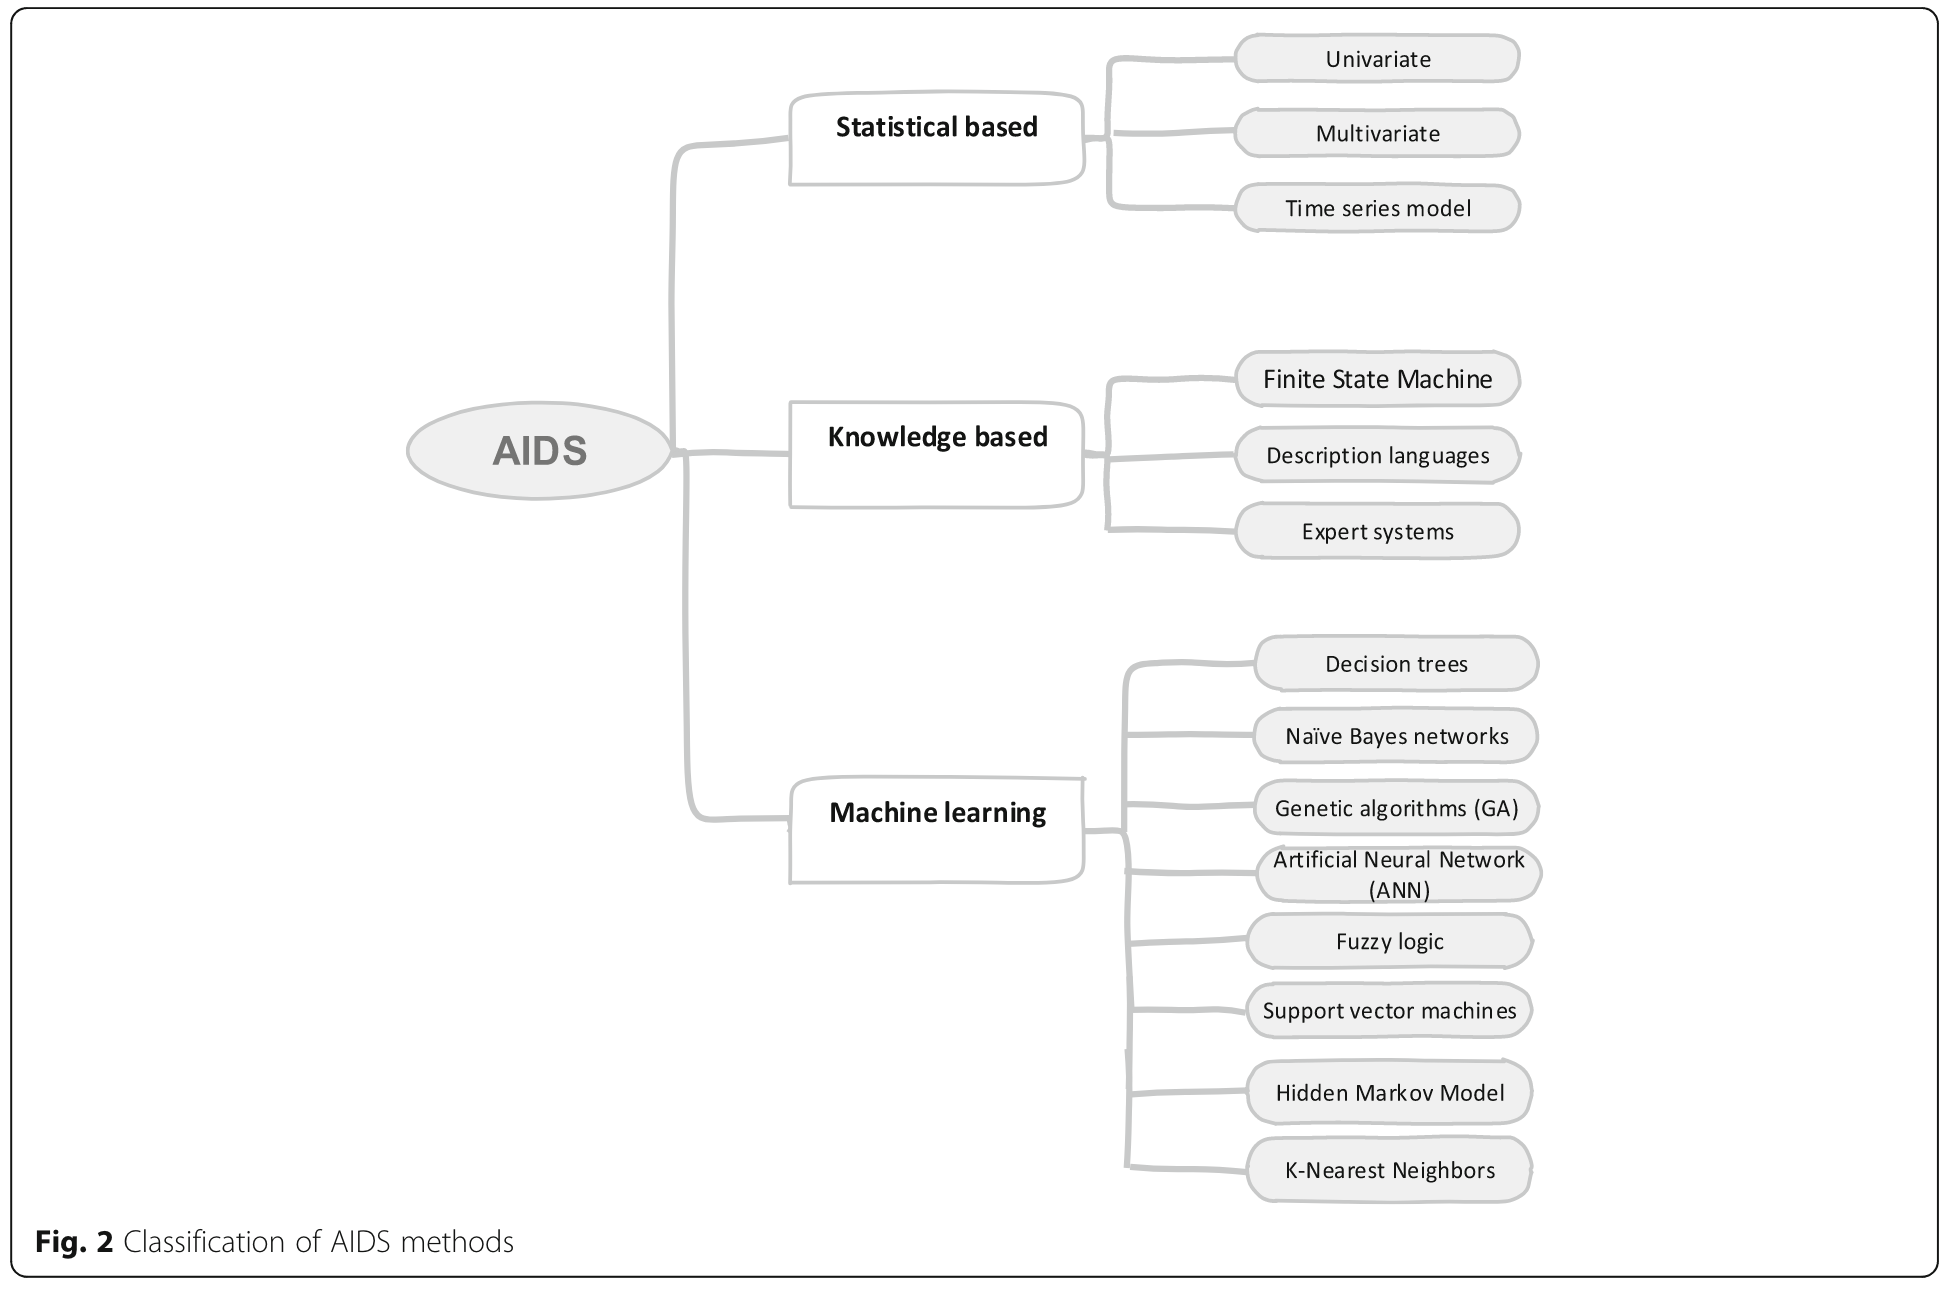
\includegraphics[width=\textwidth,height=10cm,keepaspectratio=true]{img/aids_classification.png}
    \caption{
        Schema che riassume i vari metodi di implementazione degli AIDS, da \cite{SurveyIntrusionDetection2019}. I modelli sono divisi nelle tre categorie descritte precedentemente, ma sono presenti anche i vari tipi di algoritmi utilizzati.
    }
    \label{fig:aids_classification}
\end{figure}


\subsection{Stateful-Protocol-Analysis}

In questo caso gli IDS conoscono lo stato e le specifiche del protocollo utilizzato. Vengono quindi rilevati degli eventi che non rispettano gli standard del protocollo, generalmente quelli da specifica e.g. IEEE.

Potrebbe sembrare che gli AD e gli SPA siano simili, in realtà i primi, conoscono il comportamento di una specifica rete,  mentre i secondi, conoscono solo gli standard dei protocolli.



\section{Machine Learning per rilevamento di intrusioni}


\subsection{Machine Learning}

Il Machine Learning (ML) è un sottoinsieme dell'intelligenza artificiale che permette ai sistemi di imparare da dati e di migliorare le loro prestazioni nel tempo senza essere esplicitamente programmati. Nel caso degli Intrusion Detection Systems, gli algoritmi di ML permettono di rilevare in maniera precisa e rapida attacchi per grandi quantità di dati in poco tempo ~\cite{saranyaPerformanceAnalysisMachine2020}.


Solitamente gli questi algoritmi sono divisi in:


\begin{itemize}
    \item Supervised
    \item Unsupervised 
    \item Semi-supervised
\end{itemize}

Inoltre gli algoritmi di ML possono essere usati per la classificazione o per la predizione.

La classificazione è un problema di apprendimento, in cui il modello viene addestrato su un dataset con classi conosciute e cerca di trovare una relazione tra le caratteristiche dei dati e le classi stesse. 
Un classificatore mappa una funzione: 

\[
f(x_1,\ldots x_S) = \hat y
\]

che assegna uno scalare, facente parte di un insieme $C$ di elementi disgiunti (le classi), ad un insieme di $S$ elementi vettoriali (le caratteristiche). ~\cite{hoffmannBenchmarkingClassificationRegression2019}


Nella regressione invece, si cerca di approssimare la funzione: 

\[
f(x_1,\ldots x_S) = y
\]

a partire dalle caratteristiche. La funzione $f$ è approssimata utilizzando varie tecniche di interpolazione, estrapolazione, analisi di regressione e curve fitting. ~\cite{hoffmannBenchmarkingClassificationRegression2019}



\subsubsection{Supervised Machine Learning}

Il Supervised Machine Learning utilizza un dataset con classi completamente etichettate cercando di trovare una relazione tra gli elementi del dataset e le classi di questi dati. 
La classificazione è composta da due parti: l'addestramento e il test. L'addestramento utilizza una variabile di controllo, mentre nel test, si fa predire parte del dataset al modello controllando poi i risultati. Ci sono vari algoritmi di questo tipo e.g. Support Vector Machine (SVM), Naïve Bayes, Reti Neurali, Alberi di Decisione, Random Fores.


\subsubsection{Unsupervised Machine Learning}

In questo caso, gli algoritmi di ML non hanno un dataset con classi etichettate. Questi algoritmi cercano di trovare delle relazioni tra i dati, cercando di raggrupparli in base a delle caratteristiche comuni.

L'unsupervised machine learning mostra però basse prestazioni per quanto riguarda il rilevamento quindi non possono essere utilizzati come principale strunento per gli IDS. Il motivo di questo scarso rendimento è dovuto al fatto che è molto probabile generare dei Falsi Positivi (vengono rilevati attacchi quando in realtà non cene sono) oppure generare dei Falsi Negativi (non venongo rilevati attacchi quando in realtà ce ne sono) questo va a degradare le performance generali del modello. ~\cite{UnsupervisedAlgorithmsDetect2021} 

D'altra parte però questi modelli si sono dimostrati opinabilmente migliori per rilveare gli attacchi zero-day. ~\cite{UnsupervisedAlgorithmsDetect2021}




\section{XGboost}


\section{Dataset}


